\documentclass{article}
\author{Alejandro Zubiri}
\date{Thu Oct 10 2024}
\title{Dinámica}

\usepackage{amsmath}
\usepackage{amsthm}
\usepackage{physics}
\usepackage{tikz}
\usepackage{slashed}

\newtheorem*{newton_first}{Definición}
\newtheorem*{newton_second}{Definición}
\newtheorem*{newton_third}{Definición}

\begin{document}
\maketitle
\tableofcontents
\pagebreak
La dinámica es el estudio de las fuerzas. Definimos como fuerza una interacción que cambia el estado del movimiento de
un determinado objeto.
\section{Interacciones fundamentales}
Las interacciones fundamentales son todas aquellas que hacen que el universo se comporta tal y como lo hace.
En la actualidad, se entienden cuatro interacciones:
\begin{itemize}
    \item \textbf{Gravedad}: En la física clásica, es aquella fuerza entre dos objetos, y es la que hace que algo se caiga
    hacia el centro de la Tierra cuando lo soltamos. En la actualidad, la gravedad no es una fuerza, y se describe, gracias a
    la teoría de la Relatividad General de Einstein, como la curvatura del propio espacio-tiempo.
    \item \textbf{Electromagnética}: es la responsable de la atracción y respulsión entre protones y electrones, y
    es mucho más "fuerte" a la gravedad. Esta interacción es la más habitual, responsable de que nosotros no seamos
    capaces de atravesar otros objetos. Esta, junto con las interacciones nucleares, se describe por la mecánica
    cuántica, a diferencia de la gravedad.
    \item \textbf{Fuerza nuclear fuerte}: es la responsable de mantener unidas los neutrones y protones, y la que hace
    que las propias partículas que conforman los protones (cuarks) se mantengan unidas.
    \item \textbf{Fuerza nuclear débil}: es la responsable de la mayoría de procesos de desintegración nuclear.
\end{itemize}
\section{Leyes de Newton}
\begin{newton_first}[1ra ley de Newton]
    Si no se actua ninguna fuerza sobre un cuerpo, su velocidad se mantiene constante.
\end{newton_first}
\begin{newton_second}[2da ley de Newton]
    La tasa de cambio del momento de una partícula es igual al sumatorio de todas las fuerzas que actuan en ella.
    \begin{equation}
        \begin{split}
            \sum \vec{F}= \dv{\vec{p}}{t}=m\vec{a}
        \end{split}
    \end{equation}
    Respecto a las fuerzas fundamentales, se entiende una fuerza como
    \begin{equation}
        \begin{split}
            \vec{F}= \vec{\nabla} U
        \end{split}
    \end{equation}
    Donde $U$ es el potencial de dicha fuerza
\end{newton_second}
\begin{newton_third}[3ra ley de Newton]
    Para cada fuerza ejercida hay una fuerza de igual magnitudo en sentido
    contrario. Esto es consecuencia de la \textbf{conservación de momento
    lineal}.
    \begin{equation}
        \begin{split}
            \dv{p}{t} = 0
        \end{split}
    \end{equation}
\end{newton_third}
\section{Situaciones físicas}
Estudiaremos diferentes situaciones. Para notación, utilizaremos:
\begin{itemize}
    \item $\vec{F}$: fuerza genérica ejercida a menos que se especifique.
    \item $\vec{F_{r}}$: fuerza de rozamiento.
    \item $\vec{P}=m \vec{g}$: peso.
    \item $\vec{N}$: fuerza normal.
\end{itemize}
\subsection{Plano inclinado}


\tikzset{every picture/.style={line width=0.75pt}} %set default line width to 0.75pt        

\begin{tikzpicture}[x=0.75pt,y=0.75pt,yscale=-1,xscale=1]
%uncomment if require: \path (0,300); %set diagram left start at 0, and has height of 300

%Straight Lines [id:da7727366531185051] 
\draw    (161,151.6) -- (459,151.6) ;
%Shape: Rectangle [id:dp44095981769907455] 
\draw   (273,112) -- (343,112) -- (343,152) -- (273,152) -- cycle ;
%Straight Lines [id:da25151971255607] 
\draw    (308,132) -- (406,132) ;
\draw [shift={(408,132)}, rotate = 180] [color={rgb, 255:red, 0; green, 0; blue, 0 }  ][line width=0.75]    (10.93,-3.29) .. controls (6.95,-1.4) and (3.31,-0.3) .. (0,0) .. controls (3.31,0.3) and (6.95,1.4) .. (10.93,3.29)   ;
%Straight Lines [id:da5424921835854755] 
\draw    (308,132) -- (210,132) ;
\draw [shift={(208,132)}, rotate = 360] [color={rgb, 255:red, 0; green, 0; blue, 0 }  ][line width=0.75]    (10.93,-3.29) .. controls (6.95,-1.4) and (3.31,-0.3) .. (0,0) .. controls (3.31,0.3) and (6.95,1.4) .. (10.93,3.29)   ;
%Shape: Axis 2D [id:dp7650909026809889] 
\draw  (124.3,151.6) -- (491.3,151.6)(161,16.6) -- (161,166.6) (484.3,146.6) -- (491.3,151.6) -- (484.3,156.6) (156,23.6) -- (161,16.6) -- (166,23.6)  ;
%Straight Lines [id:da9543986950239483] 
\draw    (308,132) -- (308,78.6) ;
\draw [shift={(308,76.6)}, rotate = 90] [color={rgb, 255:red, 0; green, 0; blue, 0 }  ][line width=0.75]    (10.93,-3.29) .. controls (6.95,-1.4) and (3.31,-0.3) .. (0,0) .. controls (3.31,0.3) and (6.95,1.4) .. (10.93,3.29)   ;
%Straight Lines [id:da983128628153376] 
\draw    (308,132) -- (308,190.6) ;
\draw [shift={(308,192.6)}, rotate = 270] [color={rgb, 255:red, 0; green, 0; blue, 0 }  ][line width=0.75]    (10.93,-3.29) .. controls (6.95,-1.4) and (3.31,-0.3) .. (0,0) .. controls (3.31,0.3) and (6.95,1.4) .. (10.93,3.29)   ;

% Text Node
\draw (396,105.4) node [anchor=north west][inner sep=0.75pt]    {$\vec{F}$};
% Text Node
\draw (211,100.4) node [anchor=north west][inner sep=0.75pt]    {$\overrightarrow{F_{r}}$};
% Text Node
\draw (301,40.4) node [anchor=north west][inner sep=0.75pt]    {$\vec{N}$};
% Text Node
\draw (294,196.4) node [anchor=north west][inner sep=0.75pt]    {$m\vec{g}$};


\end{tikzpicture}
Dividiremos los dos ejes:
\begin{equation}
    \begin{split}
        \sum F_{x}=F-F_{r}=ma_{x}
    \end{split}
\end{equation}
\begin{equation}
    \begin{split}
        \sum F_{y}=N-mg=0
    \end{split}
\end{equation}
La fuerza total es $0$ porque no se mueve en el eje Y.
\begin{equation}
    \begin{split}
        F_{r}=\mu N=\mu mg
    \end{split}
\end{equation}
\begin{equation}
    \begin{split}
        a_{x}=\frac{F}{m}-\mu g
    \end{split}
\end{equation}
\subsection{Plano inclinado}
\begin{center}
    

\tikzset{every picture/.style={line width=0.75pt}} %set default line width to 0.75pt        

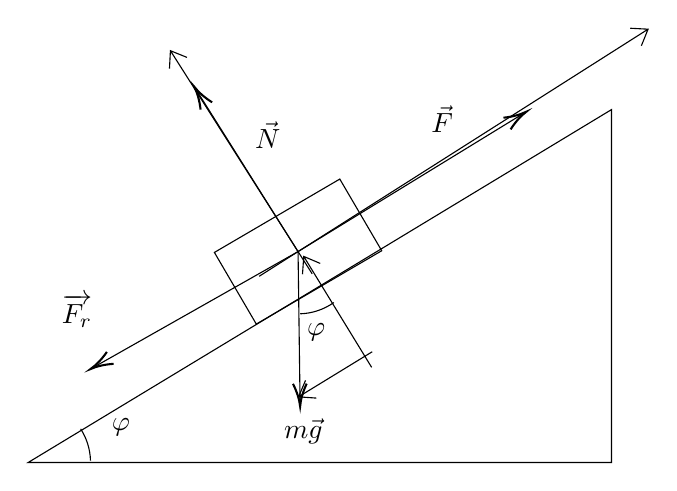
\begin{tikzpicture}[x=0.75pt,y=0.75pt,yscale=-1,xscale=1]
%uncomment if require: \path (0,300); %set diagram left start at 0, and has height of 300

%Shape: Right Triangle [id:dp325120907129558] 
\draw   (468,63.6) -- (187,233.6) -- (468,233.6) -- cycle ;
%Shape: Rectangle [id:dp7616503213503554] 
\draw   (276.69,132.41) -- (337.11,97.06) -- (357.31,131.59) -- (296.89,166.94) -- cycle ;
%Shape: Arc [id:dp6163171131169443] 
\draw  [draw opacity=0] (212.26,217.41) .. controls (215.11,221.85) and (216.83,227.09) .. (216.99,232.72) -- (187,233.6) -- cycle ; \draw   (212.26,217.41) .. controls (215.11,221.85) and (216.83,227.09) .. (216.99,232.72) ;  
%Straight Lines [id:da06147664569756994] 
\draw    (317,132) -- (425.29,65.64) ;
\draw [shift={(427,64.6)}, rotate = 148.5] [color={rgb, 255:red, 0; green, 0; blue, 0 }  ][line width=0.75]    (10.93,-3.29) .. controls (6.95,-1.4) and (3.31,-0.3) .. (0,0) .. controls (3.31,0.3) and (6.95,1.4) .. (10.93,3.29)   ;
%Straight Lines [id:da1587001463642952] 
\draw    (317,132) -- (218.74,187.61) ;
\draw [shift={(217,188.6)}, rotate = 330.49] [color={rgb, 255:red, 0; green, 0; blue, 0 }  ][line width=0.75]    (10.93,-3.29) .. controls (6.95,-1.4) and (3.31,-0.3) .. (0,0) .. controls (3.31,0.3) and (6.95,1.4) .. (10.93,3.29)   ;
%Straight Lines [id:da6647490327702699] 
\draw    (317,132) -- (268.07,54.29) ;
\draw [shift={(267,52.6)}, rotate = 57.8] [color={rgb, 255:red, 0; green, 0; blue, 0 }  ][line width=0.75]    (10.93,-3.29) .. controls (6.95,-1.4) and (3.31,-0.3) .. (0,0) .. controls (3.31,0.3) and (6.95,1.4) .. (10.93,3.29)   ;
%Straight Lines [id:da027829464308124274] 
\draw    (317,132) -- (317.97,204.6) ;
\draw [shift={(318,206.6)}, rotate = 269.23] [color={rgb, 255:red, 0; green, 0; blue, 0 }  ][line width=0.75]    (10.93,-3.29) .. controls (6.95,-1.4) and (3.31,-0.3) .. (0,0) .. controls (3.31,0.3) and (6.95,1.4) .. (10.93,3.29)   ;
%Shape: Axis 2D [id:dp8713038005007958] 
\draw  (298.26,143.91) -- (485.64,24.85)(255.51,35.22) -- (323.83,142.75) (477.05,24.39) -- (485.64,24.85) -- (482.41,32.83) (255.05,43.81) -- (255.51,35.22) -- (263.49,38.45)  ;
%Shape: Axis 2D [id:dp11883279802429425] 
\draw  (352.73,180.26) -- (317.24,201.98)(319.75,134.34) -- (352.45,187.77) (320.6,194.06) -- (317.24,201.98) -- (325.82,202.59) (327.67,137.7) -- (319.75,134.34) -- (319.14,142.92)  ;
%Shape: Arc [id:dp1720431201874566] 
\draw  [draw opacity=0] (334.26,156.54) .. controls (329.64,159.79) and (324.07,161.78) .. (318.05,161.98) -- (317,132) -- cycle ; \draw   (334.26,156.54) .. controls (329.64,159.79) and (324.07,161.78) .. (318.05,161.98) ;  

% Text Node
\draw (226,211.4) node [anchor=north west][inner sep=0.75pt]    {$\varphi $};
% Text Node
\draw (202,151.4) node [anchor=north west][inner sep=0.75pt]    {$\overrightarrow{F_{r}}$};
% Text Node
\draw (309,211.4) node [anchor=north west][inner sep=0.75pt]    {$m\vec{g}$};
% Text Node
\draw (295,68.4) node [anchor=north west][inner sep=0.75pt]    {$\vec{N}$};
% Text Node
\draw (380,60.4) node [anchor=north west][inner sep=0.75pt]    {$\vec{F}$};
% Text Node
\draw (320.05,165.38) node [anchor=north west][inner sep=0.75pt]    {$\varphi $};


\end{tikzpicture}
\end{center}
Dividimos el peso en componentes:
\begin{equation}
    \begin{split}
        P_{x}=-mg\sin \varphi\\
        P_{y}=-mg\cos \varphi
    \end{split}
\end{equation}
Y dividimos cada eje de nuevo
\begin{equation}
    \begin{split}
        \sum F_{y}=N-mg\cos \varphi = 0
    \end{split}
\end{equation}
\begin{equation}
    \begin{split}
        \sum F_{x}=F-\mu mg \sin \varphi=ma_{x}
    \end{split}
\end{equation}
\subsection{Máquina de Atwood}
\begin{center}


    \tikzset{every picture/.style={line width=0.75pt}} %set default line width to 0.75pt        

    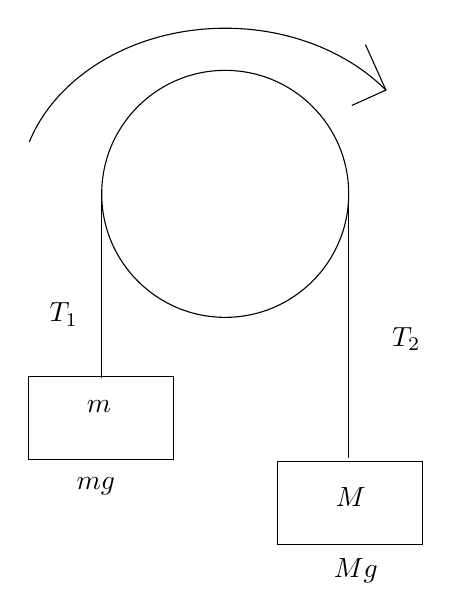
\begin{tikzpicture}[x=0.75pt,y=0.75pt,yscale=-1,xscale=1]
    %uncomment if require: \path (0,300); %set diagram left start at 0, and has height of 300
    
    %Shape: Circle [id:dp7737801781697402] 
    \draw   (235.4,85.1) .. controls (235.4,52.24) and (262.04,25.6) .. (294.9,25.6) .. controls (327.76,25.6) and (354.4,52.24) .. (354.4,85.1) .. controls (354.4,117.96) and (327.76,144.6) .. (294.9,144.6) .. controls (262.04,144.6) and (235.4,117.96) .. (235.4,85.1) -- cycle ;
    %Straight Lines [id:da025761516558777453] 
    \draw    (235.4,85.1) -- (235.4,173.6) ;
    %Straight Lines [id:da553485289140063] 
    \draw    (354.4,85.1) -- (354.4,212.6) ;
    %Shape: Rectangle [id:dp7747968036147903] 
    \draw   (200,173) -- (270,173) -- (270,213) -- (200,213) -- cycle ;
    %Shape: Rectangle [id:dp10621037288958513] 
    \draw   (320,214) -- (390,214) -- (390,254) -- (320,254) -- cycle ;
    %Shape: Arc [id:dp3739129478575194] 
    \draw  [draw opacity=0] (200.5,60.12) .. controls (213.55,28.28) and (250.88,5.3) .. (294.9,5.3) .. controls (326.21,5.3) and (354.13,16.93) .. (372.34,35.1) -- (294.9,85.1) -- cycle ; \draw   (200.5,60.12) .. controls (213.55,28.28) and (250.88,5.3) .. (294.9,5.3) .. controls (326.21,5.3) and (354.13,16.93) .. (372.34,35.1) ;  
    %Shape: Right Angle [id:dp5937175858339385] 
    \draw   (362.46,13.18) -- (372.34,35.1) -- (355.88,42.52) ;
    
    % Text Node
    \draw (227,183.4) node [anchor=north west][inner sep=0.75pt]    {$m$};
    % Text Node
    \draw (347,225.4) node [anchor=north west][inner sep=0.75pt]    {$M$};
    % Text Node
    \draw (209,136.4) node [anchor=north west][inner sep=0.75pt]    {$T_{1}$};
    % Text Node
    \draw (374,148.4) node [anchor=north west][inner sep=0.75pt]    {$T_{2}$};
    % Text Node
    \draw (222,220.4) node [anchor=north west][inner sep=0.75pt]    {$mg$};
    % Text Node
    \draw (346,259.4) node [anchor=north west][inner sep=0.75pt]    {$Mg$};
    
    
    \end{tikzpicture}
\end{center}
Consideramos el eje positivo el sentido horario.
\begin{equation}
    \begin{split}
        \sum F_{1}=T_{1}-mg=ma_{1}\\
        \sum F_{2}=-T_{2}+Mg
    \end{split}
\end{equation}
Como la cuerda no se extiende ni contrae, ambas tensiones son iguales, y ambas aceleraciones también:
\begin{equation}
    \begin{split}
        T_{1}=T_{2}\\
        a_{1}=a_{2}
    \end{split}
\end{equation}
Obteniendo así que
\begin{equation}
    \begin{split}
        a(M+m)=g(M-m)
    \end{split}
\end{equation}
\begin{equation}
    \begin{split}
        a= g \frac{M-m}{M+m}
    \end{split}
\end{equation}
\subsection{Péndulo Cónico}
\begin{center}
    

\tikzset{every picture/.style={line width=0.75pt}} %set default line width to 0.75pt        

\begin{tikzpicture}[x=0.75pt,y=0.75pt,yscale=-1,xscale=1]
%uncomment if require: \path (0,300); %set diagram left start at 0, and has height of 300

%Shape: Ellipse [id:dp9496159632670964] 
\draw  [dash pattern={on 4.5pt off 4.5pt}] (217,184.8) .. controls (217,160.06) and (256.85,140) .. (306,140) .. controls (355.15,140) and (395,160.06) .. (395,184.8) .. controls (395,209.54) and (355.15,229.6) .. (306,229.6) .. controls (256.85,229.6) and (217,209.54) .. (217,184.8) -- cycle ;
%Straight Lines [id:da272805244293052] 
\draw  [dash pattern={on 4.5pt off 4.5pt}]  (306,48.6) -- (306,184.8) ;
%Straight Lines [id:da2791426433208275] 
\draw    (306,48.6) -- (395,184.8) ;
%Shape: Arc [id:dp33240302819847467] 
\draw  [draw opacity=0] (321.9,74.04) .. controls (317.29,76.93) and (311.84,78.6) .. (306,78.6) .. controls (305.79,78.6) and (305.58,78.6) .. (305.38,78.59) -- (306,48.6) -- cycle ; \draw   (321.9,74.04) .. controls (317.29,76.93) and (311.84,78.6) .. (306,78.6) .. controls (305.79,78.6) and (305.58,78.6) .. (305.38,78.59) ;  
%Straight Lines [id:da20364655882605964] 
\draw    (217,184.8) -- (306,184.8) ;
%Straight Lines [id:da49122186904394205] 
\draw    (395,184.8) -- (395,146.6) ;
\draw [shift={(395,144.6)}, rotate = 90] [color={rgb, 255:red, 0; green, 0; blue, 0 }  ][line width=0.75]    (10.93,-3.29) .. controls (6.95,-1.4) and (3.31,-0.3) .. (0,0) .. controls (3.31,0.3) and (6.95,1.4) .. (10.93,3.29)   ;
%Straight Lines [id:da8865676315985294] 
\draw    (395,184.8) -- (350,184.8) ;
\draw [shift={(348,184.8)}, rotate = 360] [color={rgb, 255:red, 0; green, 0; blue, 0 }  ][line width=0.75]    (10.93,-3.29) .. controls (6.95,-1.4) and (3.31,-0.3) .. (0,0) .. controls (3.31,0.3) and (6.95,1.4) .. (10.93,3.29)   ;
%Straight Lines [id:da7115687840837579] 
\draw    (395,184.8) -- (395,246.5) ;
\draw [shift={(395,248.5)}, rotate = 270] [color={rgb, 255:red, 0; green, 0; blue, 0 }  ][line width=0.75]    (10.93,-3.29) .. controls (6.95,-1.4) and (3.31,-0.3) .. (0,0) .. controls (3.31,0.3) and (6.95,1.4) .. (10.93,3.29)   ;
%Straight Lines [id:da1404326978598136] 
\draw  [dash pattern={on 4.5pt off 4.5pt}]  (394,233.6) -- (439,233.6) ;
%Straight Lines [id:da4237844082525637] 
\draw  [dash pattern={on 4.5pt off 4.5pt}]  (439,233.6) -- (395,184.8) ;
%Shape: Arc [id:dp07940826347657137] 
\draw  [draw opacity=0] (405.97,197.31) .. controls (403.15,200.23) and (399.64,202.43) .. (395.72,203.61) -- (389,179.7) -- cycle ; \draw   (405.97,197.31) .. controls (403.15,200.23) and (399.64,202.43) .. (395.72,203.61) ;  
%Straight Lines [id:da9065869061524914] 
\draw  [dash pattern={on 4.5pt off 4.5pt}]  (394,233.6) -- (350,184.8) ;
%Shape: Arc [id:dp831375371933305] 
\draw  [draw opacity=0] (383.31,224.19) .. controls (386.61,221.31) and (390.88,219.43) .. (395.61,219.07) -- (397.3,238.75) -- cycle ; \draw   (383.31,224.19) .. controls (386.61,221.31) and (390.88,219.43) .. (395.61,219.07) ;  

% Text Node
\draw (307.38,81.99) node [anchor=north west][inner sep=0.75pt]    {$\phi $};
% Text Node
\draw (252,164.4) node [anchor=north west][inner sep=0.75pt]    {$r$};
% Text Node
\draw (390,115.4) node [anchor=north west][inner sep=0.75pt]    {$a_{t}$};
% Text Node
\draw (343,160.4) node [anchor=north west][inner sep=0.75pt]    {$F_{n}$};
% Text Node
\draw (384,244.4) node [anchor=north west][inner sep=0.75pt]    {$mg$};
% Text Node
\draw (399.38,201.99) node [anchor=north west][inner sep=0.75pt]    {$\phi $};
% Text Node
\draw (380.38,202.99) node [anchor=north west][inner sep=0.75pt]    {$\phi $};


\end{tikzpicture}
\end{center}
En este caso, contamos con velocidad angular constante, $a_{t}=0$.\\
Si observamos el triángulo inferior, podemos observar una relación entre el ángulo $\phi $,
el peso $mg$, y la fuerza normal $F_{n}$. Teniendo en cuenta que $r=l\sin \phi $:
\begin{equation}
    \begin{split}
        \tan \phi = \frac{F_{n}}{mg}= \frac{m \frac{v^{2}}{r}}{mg}= \frac{v^{2}}{gr}=
        \frac{\omega ^{2}r}{g}= \frac{\omega^{2}\sin \phi l}{g}
    \end{split}
\end{equation}
\begin{equation}
    \begin{split}
            \tan \phi &= \frac{\omega^{2}\sin \phi l}{g}\\
            \frac{\sin \phi }{\cos \phi } &= \frac{\omega^{2}\sin \phi l}{g}\\
            \frac{1}{\cos \phi } &= \frac{\omega^{2} l}{g}\\
            \cos \phi &= \frac{g}{\omega^{2}l}
    \end{split}
\end{equation}
\subsection{Superfície Semiesférica}
\begin{center}
    

\tikzset{every picture/.style={line width=0.75pt}} %set default line width to 0.75pt        

\begin{tikzpicture}[x=0.75pt,y=0.75pt,yscale=-1,xscale=1]
%uncomment if require: \path (0,300); %set diagram left start at 0, and has height of 300

%Straight Lines [id:da8314996879472738] 
\draw  [dash pattern={on 4.5pt off 4.5pt}]  (200,111) -- (481,111) ;
%Shape: Arc [id:dp5384099731909817] 
\draw  [draw opacity=0] (481,111) .. controls (478.25,186.18) and (416.44,246.28) .. (340.6,246.28) .. controls (263.94,246.28) and (201.62,184.89) .. (200.12,108.6) -- (340.6,105.78) -- cycle ; \draw   (481,111) .. controls (478.25,186.18) and (416.44,246.28) .. (340.6,246.28) .. controls (263.94,246.28) and (201.62,184.89) .. (200.12,108.6) ;  
%Straight Lines [id:da058326523918503126] 
\draw    (340.5,18.6) -- (340.5,244.6) ;
%Shape: Circle [id:dp01670193335304737] 
\draw  [fill={rgb, 255:red, 0; green, 0; blue, 0 }  ,fill opacity=1 ] (207.9,166.3) .. controls (207.9,162.54) and (210.94,159.5) .. (214.7,159.5) .. controls (218.46,159.5) and (221.5,162.54) .. (221.5,166.3) .. controls (221.5,170.06) and (218.46,173.1) .. (214.7,173.1) .. controls (210.94,173.1) and (207.9,170.06) .. (207.9,166.3) -- cycle ;
%Straight Lines [id:da2019416040342772] 
\draw    (214.7,166.3) -- (340.5,111) ;
%Straight Lines [id:da9842582318013553] 
\draw  [dash pattern={on 4.5pt off 4.5pt}]  (117.6,208.5) -- (449.6,63.5) ;
%Straight Lines [id:da40119198105158227] 
\draw  [dash pattern={on 4.5pt off 4.5pt}]  (176.75,84) -- (249.33,241.39) ;
%Straight Lines [id:da9955855598791858] 
\draw    (214.7,166.3) -- (261.42,145.76) ;
\draw [shift={(263.26,144.96)}, rotate = 156.27] [color={rgb, 255:red, 0; green, 0; blue, 0 }  ][line width=0.75]    (10.93,-3.29) .. controls (6.95,-1.4) and (3.31,-0.3) .. (0,0) .. controls (3.31,0.3) and (6.95,1.4) .. (10.93,3.29)   ;
%Straight Lines [id:da6553481460065997] 
\draw    (214.7,166.3) -- (214.7,217.5) ;
\draw [shift={(214.7,219.5)}, rotate = 270] [color={rgb, 255:red, 0; green, 0; blue, 0 }  ][line width=0.75]    (10.93,-3.29) .. controls (6.95,-1.4) and (3.31,-0.3) .. (0,0) .. controls (3.31,0.3) and (6.95,1.4) .. (10.93,3.29)   ;
%Straight Lines [id:da20003156938497813] 
\draw    (214.7,219.5) -- (189.68,180.68) ;
\draw [shift={(188.6,179)}, rotate = 57.2] [color={rgb, 255:red, 0; green, 0; blue, 0 }  ][line width=0.75]    (10.93,-3.29) .. controls (6.95,-1.4) and (3.31,-0.3) .. (0,0) .. controls (3.31,0.3) and (6.95,1.4) .. (10.93,3.29)   ;

% Text Node
\draw (283.4,112.9) node [anchor=north west][inner sep=0.75pt]    {$\phi $};
% Text Node
\draw (453.4,50.4) node [anchor=north west][inner sep=0.75pt]    {$y$};
% Text Node
\draw (161.4,53.9) node [anchor=north west][inner sep=0.75pt]    {$x$};
% Text Node
\draw (203.4,226.9) node [anchor=north west][inner sep=0.75pt]    {$mg$};
% Text Node
\draw (201.9,190.4) node [anchor=north west][inner sep=0.75pt]  [font=\footnotesize]  {$\phi $};


\end{tikzpicture}
\end{center}
Vamos a dividir cada eje:
\begin{equation}
    \begin{split}
        &F_{x}=mg\cos \phi =ma_{t} \implies g\cos \phi = \dv{|v|}{t}\\
        &F_{y}=-mg\sin \phi +N=ma_{n}=m \frac{v^{2}}{r}
    \end{split}
\end{equation}
Podemos hacer unas piruetas con la primera ecuación:
\begin{equation}
    \begin{split}
        g\cos \phi = \dv{|v|}{\phi }\dv{\phi }{t}=\dv{|v|}{\phi } \frac{|v|}{r}
    \end{split}
\end{equation}
Podemos reorganizar la ecuación e integrar:
\begin{equation}
    \begin{split}
        \int gr\cos \phi \, \dd{\phi } &= \int |v|\,\dd{|v|}\\
        gr\sin \phi &= \frac{|v|^{2}}{2}\\
        |v|&=\sqrt{2rg\sin \phi }
    \end{split}
\end{equation}
Si realizamos la sustitución $v=\omega r$ y reordenamos, obtenemos que:
\begin{equation}
    \begin{split}
        t(\phi )= \sqrt{\frac{r}{2g}} \int_{0}^\phi \frac{\dd{\phi }}{\sqrt{\sin \phi }} 
    \end{split}
\end{equation}
\subsection{Curva con peralte}
\begin{center}
    

\tikzset{every picture/.style={line width=0.75pt}} %set default line width to 0.75pt        

\begin{tikzpicture}[x=0.75pt,y=0.75pt,yscale=-1,xscale=1]
%uncomment if require: \path (0,300); %set diagram left start at 0, and has height of 300

%Straight Lines [id:da6275656197385018] 
\draw    (83,192) -- (435,192) ;
%Straight Lines [id:da6643994969329394] 
\draw    (435,192) -- (86,92.6) ;
%Shape: Arc [id:dp22325641824710063] 
\draw  [draw opacity=0] (370,192.64) .. controls (370,192.42) and (370,192.21) .. (370,192) .. controls (370,185.51) and (370.95,179.23) .. (372.73,173.32) -- (435,192) -- cycle ; \draw   (370,192.64) .. controls (370,192.42) and (370,192.21) .. (370,192) .. controls (370,185.51) and (370.95,179.23) .. (372.73,173.32) ;  
%Shape: Rectangle [id:dp9299682122355795] 
\draw   (259.01,100.78) -- (326.54,119.24) -- (315.99,157.82) -- (248.46,139.36) -- cycle ;
%Straight Lines [id:da7276094732627185] 
\draw  [dash pattern={on 4.5pt off 4.5pt}]  (287.6,9) -- (287.6,252.5) ;
%Straight Lines [id:da05744723298663579] 
\draw  [dash pattern={on 4.5pt off 4.5pt}]  (145.1,130.75) -- (478.6,130.75) ;
%Straight Lines [id:da6386494764700066] 
\draw    (287.6,130.75) -- (380.68,158.43) ;
\draw [shift={(382.6,159)}, rotate = 196.56] [color={rgb, 255:red, 0; green, 0; blue, 0 }  ][line width=0.75]    (10.93,-3.29) .. controls (6.95,-1.4) and (3.31,-0.3) .. (0,0) .. controls (3.31,0.3) and (6.95,1.4) .. (10.93,3.29)   ;
%Straight Lines [id:da27506116125567437] 
\draw    (287.6,130.75) -- (315.05,34.42) ;
\draw [shift={(315.6,32.5)}, rotate = 105.91] [color={rgb, 255:red, 0; green, 0; blue, 0 }  ][line width=0.75]    (10.93,-3.29) .. controls (6.95,-1.4) and (3.31,-0.3) .. (0,0) .. controls (3.31,0.3) and (6.95,1.4) .. (10.93,3.29)   ;
%Straight Lines [id:da5004170413028757] 
\draw    (287.6,130.75) -- (287.6,222.5) ;
\draw [shift={(287.6,224.5)}, rotate = 270] [color={rgb, 255:red, 0; green, 0; blue, 0 }  ][line width=0.75]    (10.93,-3.29) .. controls (6.95,-1.4) and (3.31,-0.3) .. (0,0) .. controls (3.31,0.3) and (6.95,1.4) .. (10.93,3.29)   ;

% Text Node
\draw (335,171.4) node [anchor=north west][inner sep=0.75pt]    {$\phi $};
% Text Node
\draw (265,10.4) node [anchor=north west][inner sep=0.75pt]    {$y$};
% Text Node
\draw (487,120.9) node [anchor=north west][inner sep=0.75pt]    {$x$};
% Text Node
\draw (404,153.9) node [anchor=north west][inner sep=0.75pt]    {$Fr$};
% Text Node
\draw (301,225.9) node [anchor=north west][inner sep=0.75pt]    {$mg$};
% Text Node
\draw (334.5,11.4) node [anchor=north west][inner sep=0.75pt]    {$N$};


\end{tikzpicture}
\end{center}
Si realizamos la descomposición de las fuerzas por ejes:
\begin{equation}
    \begin{split}
        \sum F_{x} &= N \sin \phi + Fr \cos \phi =
        N \sin \phi  + N \mu \cos \phi =m a_{x} = m \frac{v^{2}}{r}\\
        \sum F_{y} &= N \cos \phi  -mg -Fr \sin \phi =
        N \cos \phi  - mg -N \mu  \sin \phi = 0 
    \end{split}
\end{equation}
Reordenando estas ecuaciones, podemos obtener que:
\begin{equation}
    \begin{split}
        N = \frac{mg}{\cos \phi  - \mu \sin \phi }
    \end{split}
\end{equation}
Y por tanto
\begin{equation}
    \begin{split}
        v = \sqrt{gr \frac{\sin \phi  + \mu  \cos \phi }{\cos \phi -\mu \sin \phi }}
    \end{split}
\end{equation}
Donde definimos esta velocidad como la velocidad máxima antes de empiece
a derrapar.
\subsection{Cuerpo en un fluido}
\begin{center}
    

\tikzset{every picture/.style={line width=0.75pt}} %set default line width to 0.75pt        

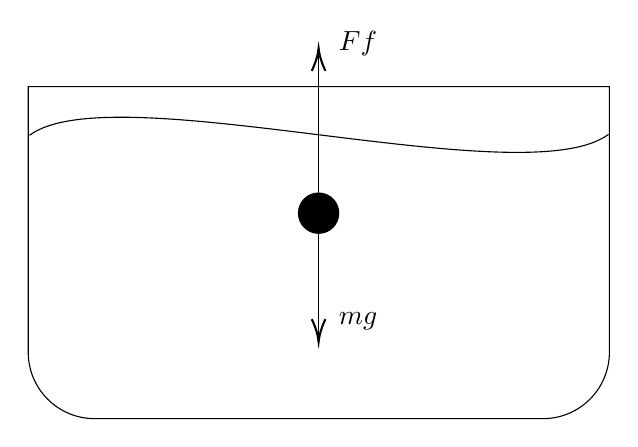
\begin{tikzpicture}[x=0.75pt,y=0.75pt,yscale=-1,xscale=1]
%uncomment if require: \path (0,300); %set diagram left start at 0, and has height of 300

%Rounded Same Side Corner Rect [id:dp033551959202890114] 
\draw   (459,188) .. controls (459,205.67) and (444.67,220) .. (427,220) -- (211,220) .. controls (193.33,220) and (179,205.67) .. (179,188) -- (179,60) .. controls (179,60) and (179,60) .. (179,60) -- (459,60) .. controls (459,60) and (459,60) .. (459,60) -- cycle ;
%Curve Lines [id:da3037365575846527] 
\draw    (179.6,83.5) .. controls (219.6,53.5) and (418.6,113) .. (458.6,83) ;
%Shape: Circle [id:dp8703676958635742] 
\draw  [fill={rgb, 255:red, 0; green, 0; blue, 0 }  ,fill opacity=1 ] (309.2,121) .. controls (309.2,115.64) and (313.54,111.3) .. (318.9,111.3) .. controls (324.26,111.3) and (328.6,115.64) .. (328.6,121) .. controls (328.6,126.36) and (324.26,130.7) .. (318.9,130.7) .. controls (313.54,130.7) and (309.2,126.36) .. (309.2,121) -- cycle ;
%Straight Lines [id:da3872629897227551] 
\draw    (318.9,111.3) -- (318.9,43.5) ;
\draw [shift={(318.9,41.5)}, rotate = 90] [color={rgb, 255:red, 0; green, 0; blue, 0 }  ][line width=0.75]    (10.93,-3.29) .. controls (6.95,-1.4) and (3.31,-0.3) .. (0,0) .. controls (3.31,0.3) and (6.95,1.4) .. (10.93,3.29)   ;
%Straight Lines [id:da4102706760637014] 
\draw    (318.9,130.7) -- (318.9,181) ;
\draw [shift={(318.9,183)}, rotate = 270] [color={rgb, 255:red, 0; green, 0; blue, 0 }  ][line width=0.75]    (10.93,-3.29) .. controls (6.95,-1.4) and (3.31,-0.3) .. (0,0) .. controls (3.31,0.3) and (6.95,1.4) .. (10.93,3.29)   ;

% Text Node
\draw (327.4,31.9) node [anchor=north west][inner sep=0.75pt]    {$Ff$};
% Text Node
\draw (327.4,167.4) node [anchor=north west][inner sep=0.75pt]    {$mg$};


\end{tikzpicture}
\end{center}
Tenemos un cuerpo de volumen $V$, de densidad $\rho $, en un fluido de
densidad $\rho _{f}$.\\
Definimos la \textbf{fuerza de flotabilidad} como
\begin{equation}
    \begin{split}
        Ff = - \kappa \eta v
    \end{split}
\end{equation}
donde
\begin{itemize}
    \item $\kappa$ es la "aerodinámica" del objeto.
    \item $\eta $ es la viscosidad del fluido.
    \item $v$ es la velocidad del objeto.
\end{itemize}
También definimos la \textbf{fuerza de empuje} del fluido como el peso
del fluido desplazado:
\begin{equation}
    \begin{split}
        E = V \rho _{f} g
    \end{split}
\end{equation}
Podemos realizar el sumatorio de fuerzas y calcular:
\begin{equation}
    \begin{split}
        F &= mg -Ff - E\\
        &= V \rho g -\kappa \eta v - V\rho _{f} g
    \end{split}
\end{equation}
\subsubsection{Velocidad en función del tiempo}:
Para simplificar la situación, podemos calcular la velocidad para un fluido
poco denso, de forma que $\rho _{f} \ll \rho $, y por tanto $\slashed{E}^0$:
\begin{equation}
    \begin{split}
        F=m a &= mg - \kappa \eta v\\
        m \dv{v}{t} &= mg -\kappa \eta v
    \end{split}
\end{equation}
Si reordenamos todo lo que está en función de $v$ y de $t$ e integramos:
\begin{equation}
    \begin{split}
        \frac{\dd{v}}{g - \frac{\kappa \eta v}{m}} &= dt\\
        \int_{v_{0}}^v \frac{\dd{v}}{g - \frac{\kappa \eta v}{m}} &=
        \int _{0}^t dt
    \end{split}
\end{equation}
Obteniendo así
\begin{equation}
    \begin{split}
        v(t) = (v_{0}- \frac{gm}{\kappa \eta })\exp(- \frac{\kappa \eta t}{m})
        + \frac{gm}{\kappa \eta }
    \end{split}
\end{equation}
También podemos calcular la velocidad límite cuando $F=0$:
\begin{equation}
    \begin{split}
        &Vg(\rho -\rho _{f})-\kappa \eta v=0\\
        & v = \frac{Vg(\rho -\rho _{f})}{\kappa \eta }
    \end{split}
\end{equation}
\section{Fuezas ficticias}
Dos sistemas son inerciales si mantienen una velocidad \textbf{constante}
entre ellos. En cambio, si aceleran entre sí, son no inerciales.\\
Las fuerzas ficticias se dan en sistemas no incerciales:
\begin{equation}
    \begin{split}
        \vec{F_{f}} = -m \vec{a}
    \end{split}
\end{equation}
\subsection{Movimiento Curvilíneo}
\begin{center}
    

\tikzset{every picture/.style={line width=0.75pt}} %set default line width to 0.75pt        

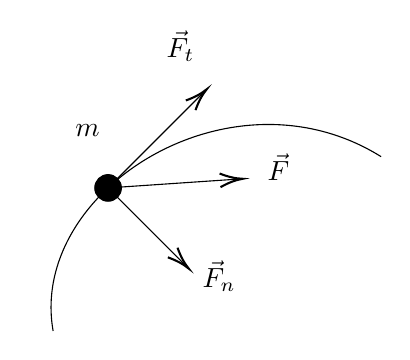
\begin{tikzpicture}[x=0.75pt,y=0.75pt,yscale=-1,xscale=1]
%uncomment if require: \path (0,300); %set diagram left start at 0, and has height of 300

%Curve Lines [id:da006742863088528228] 
\draw    (159.2,170.6) .. controls (147.2,103.27) and (244.53,41.27) .. (317.2,86.6) ;
%Shape: Circle [id:dp4851664656082346] 
\draw  [fill={rgb, 255:red, 0; green, 0; blue, 0 }  ,fill opacity=1 ] (179.27,101.67) .. controls (179.27,98.13) and (182.13,95.27) .. (185.67,95.27) .. controls (189.2,95.27) and (192.07,98.13) .. (192.07,101.67) .. controls (192.07,105.2) and (189.2,108.07) .. (185.67,108.07) .. controls (182.13,108.07) and (179.27,105.2) .. (179.27,101.67) -- cycle ;
%Straight Lines [id:da5230919627330224] 
\draw    (185.67,101.67) -- (231.79,55.55) ;
\draw [shift={(233.2,54.13)}, rotate = 135] [color={rgb, 255:red, 0; green, 0; blue, 0 }  ][line width=0.75]    (10.93,-3.29) .. controls (6.95,-1.4) and (3.31,-0.3) .. (0,0) .. controls (3.31,0.3) and (6.95,1.4) .. (10.93,3.29)   ;
%Straight Lines [id:da6826050338139313] 
\draw    (185.67,101.67) -- (223.12,139.12) ;
\draw [shift={(224.53,140.53)}, rotate = 225] [color={rgb, 255:red, 0; green, 0; blue, 0 }  ][line width=0.75]    (10.93,-3.29) .. controls (6.95,-1.4) and (3.31,-0.3) .. (0,0) .. controls (3.31,0.3) and (6.95,1.4) .. (10.93,3.29)   ;
%Straight Lines [id:da8056073149588405] 
\draw    (185.67,101.67) -- (248.54,97.4) ;
\draw [shift={(250.53,97.27)}, rotate = 176.12] [color={rgb, 255:red, 0; green, 0; blue, 0 }  ][line width=0.75]    (10.93,-3.29) .. controls (6.95,-1.4) and (3.31,-0.3) .. (0,0) .. controls (3.31,0.3) and (6.95,1.4) .. (10.93,3.29)   ;

% Text Node
\draw (168.67,69.73) node [anchor=north west][inner sep=0.75pt]    {$m$};
% Text Node
\draw (212.67,24.73) node [anchor=north west][inner sep=0.75pt]    {$\vec{F}_{t}$};
% Text Node
\draw (230,135.4) node [anchor=north west][inner sep=0.75pt]    {$\vec{F}_{n}$};
% Text Node
\draw (261.33,83.73) node [anchor=north west][inner sep=0.75pt]    {$\vec{F}$};


\end{tikzpicture}
\end{center}
Podemos descomponer esta fuerza en sus componentes tangencial y normal:
\begin{equation}
    \begin{split}
        F_{t}=m a_{t} = m \dv{|v|}{t}
    \end{split}
\end{equation}
\begin{equation}
    \begin{split}
        F_{n} = ma_{n} = m \frac{| \vec{v}|^{2}}{r}
    \end{split}
\end{equation}
\section{Momento Angular}
Definimos la magnitud vectorial del momento angular $L$ como:
\begin{equation}
    \begin{split}
        \vec{L} = \vec{r} \times \vec{p} = m \vec{r} \times \vec{v}
    \end{split}
\end{equation}
Si sustituimos nuestras ecuaciones del movimiento circular, tenemos que
\begin{equation}
    \begin{split}
        \vec{L} = m \vec{r} \times \vec{v} = m\omega r^{2} \vec{u}_n \times \vec{u}_t
        = m\omega r^{2} \vec{u}_z
    \end{split}
\end{equation}
Para ver como cambia el momento angular respecto al tiempo:
\begin{equation}
    \begin{split}
        \dv{\vec{L}}{t} &= m (\dv{\vec{r}}{t} \times \vec{v} + \vec{r}\times \dv{\vec{v}}{t})\\
        &= m \vec{v} \times \vec{v} = m\vec{r} \times \vec{a}\\
        &= \vec{r} \times \vec{F}
    \end{split}
\end{equation}
Esta última cantidad, la definimos como la \textbf{torsión}:
\begin{equation}
    \begin{split}
        \dv{\vec{L}}{t} = \vec{\tau }= \vec{r} \times \vec{F}
    \end{split}
\end{equation}
\subsection{Fuerzas centrales o radiales}
Son fuerzas que son paralelas al vector posición $\vec{r}$:
\begin{equation}
    \begin{split}
        \vec{F}_{r} \propto \vec{u}_r
    \end{split}
\end{equation}
En estos casos, la torsión es igual a $0$:
\begin{equation}
    \begin{split}
        \vec{\tau }= \vec{r} \times \vec{F}_r = \vec{r} \times r \vec{u}_r = 0
    \end{split}
\end{equation}
\section{Trabajo y energía}
\subsection{Impulso mecánico}
Definimos el impulso como el cambio en el momento:
\begin{equation}
    \begin{split}
        \vec{I}= \Delta \vec{p} = \int \vec{F} \dd{t}
    \end{split}
\end{equation}
Por tanto, definimos la posición como:
\begin{equation}
    \begin{split} 
        \vec{r} = \frac{1}{m} \vec{p}t = \vec{r}_{0} +\vec{v}_{0} t+ \int \frac{\vec{I}}{m} \dd{t}
    \end{split}
\end{equation}
\subsection{Trabajo}
\begin{center}
    

\tikzset{every picture/.style={line width=0.75pt}} %set default line width to 0.75pt        

\begin{tikzpicture}[x=0.75pt,y=0.75pt,yscale=-1,xscale=1]
%uncomment if require: \path (0,300); %set diagram left start at 0, and has height of 300

%Curve Lines [id:da8909791042207142] 
\draw    (105.87,201.47) .. controls (97.2,110.8) and (217.2,42.13) .. (303.2,74.13) ;
%Shape: Circle [id:dp500164503914132] 
\draw  [fill={rgb, 255:red, 0; green, 0; blue, 0 }  ,fill opacity=1 ] (139.47,112.33) .. controls (139.47,110.38) and (141.05,108.8) .. (143,108.8) .. controls (144.95,108.8) and (146.53,110.38) .. (146.53,112.33) .. controls (146.53,114.28) and (144.95,115.87) .. (143,115.87) .. controls (141.05,115.87) and (139.47,114.28) .. (139.47,112.33) -- cycle ;
%Straight Lines [id:da6936753450735018] 
\draw    (143,112.33) -- (203.87,112.33) ;
\draw [shift={(205.87,112.33)}, rotate = 180] [color={rgb, 255:red, 0; green, 0; blue, 0 }  ][line width=0.75]    (10.93,-3.29) .. controls (6.95,-1.4) and (3.31,-0.3) .. (0,0) .. controls (3.31,0.3) and (6.95,1.4) .. (10.93,3.29)   ;
%Straight Lines [id:da1578191418506727] 
\draw    (143,112.33) -- (159.17,94.93) ;
\draw [shift={(160.53,93.47)}, rotate = 132.9] [color={rgb, 255:red, 0; green, 0; blue, 0 }  ][line width=0.75]    (10.93,-3.29) .. controls (6.95,-1.4) and (3.31,-0.3) .. (0,0) .. controls (3.31,0.3) and (6.95,1.4) .. (10.93,3.29)   ;
%Straight Lines [id:da9324796481206004] 
\draw  [dash pattern={on 4.5pt off 4.5pt}]  (143,112.33) -- (203.12,52.21) ;
\draw [shift={(204.53,50.8)}, rotate = 135] [color={rgb, 255:red, 0; green, 0; blue, 0 }  ][line width=0.75]    (10.93,-3.29) .. controls (6.95,-1.4) and (3.31,-0.3) .. (0,0) .. controls (3.31,0.3) and (6.95,1.4) .. (10.93,3.29)   ;
%Straight Lines [id:da2907186400629769] 
\draw  [dash pattern={on 4.5pt off 4.5pt}]  (143,112.33) -- (93.95,63.28) ;
\draw [shift={(92.53,61.87)}, rotate = 45] [color={rgb, 255:red, 0; green, 0; blue, 0 }  ][line width=0.75]    (10.93,-3.29) .. controls (6.95,-1.4) and (3.31,-0.3) .. (0,0) .. controls (3.31,0.3) and (6.95,1.4) .. (10.93,3.29)   ;

% Text Node
\draw (212.67,110.4) node [anchor=north west][inner sep=0.75pt]    {$\vec{F}$};
% Text Node
\draw (132.67,71.4) node [anchor=north west][inner sep=0.75pt]    {$\overrightarrow{dr}$};
% Text Node
\draw (194.67,21.4) node [anchor=north west][inner sep=0.75pt]    {$\vec{F}_{t}$};
% Text Node
\draw (82,89.73) node [anchor=north west][inner sep=0.75pt]    {$\vec{F}_{n}$};


\end{tikzpicture}
\end{center}
Definimos el trabajo como la el producto de la fuerza con la posición a lo largo de la trayectoria
entre un punto $A$ y un punto $B$:
\begin{equation}
    \begin{split}
        \dd{W} = \vec{F}\cdot \vec{ \dd{r}} = F_{t} \dd{r} = F \dd{r} \cos \theta 
    \end{split}
\end{equation}
Podemos calcular el trabajo mediante una \textbf{integral de línea} a lo largo de toda la
trayectoria:
\begin{equation}\tag*{$[W]=J$}
    \begin{split}
        W = \int_{A}^B \vec{F}\cdot  \vec{\dd{r}}
    \end{split}
\end{equation}
\subsection{Potencia}
Definimos la potencia como el cambio en el trabajo con respecto al tiempo:
\begin{equation}
    \begin{split}
        P= \dv{W}{t} = \frac{\vec{F}\cdot \dd{r}}{ \dd{t}}= \vec{F}\cdot \vec{v}
    \end{split}
\end{equation}
La unidad de la potencia es el \textbf{watt}, definido como:
\begin{equation}
    \begin{split}
        w = kg \frac{m^{2}}{s^{3}}
    \end{split}
\end{equation}
Además, existen las siguientes comunes unidades para la potencia:
\begin{itemize}
    \item $1cv = 745w$ (Potencia)
    \item $1kwh = 3.6 \cdot 10^{6}(J)$ (Trabajo)
\end{itemize}
\subsection{Energía cinética}
Definimos la energía cinética como la energía de un sistema a causa de su movimiento:
\begin{equation}
    \begin{split}
        \dd{W} = \vec{v} \dd{\vec{p}}
    \end{split}
\end{equation}
\begin{equation}
    \begin{split}
        W = m \int_{v_{0}}^v v \dd{v} = \frac{1}{2} m \Delta v^{2} = T
    \end{split}
\end{equation}
\begin{equation}
    \begin{split}
        T = \frac{1}{2} m v^{2}
    \end{split}
\end{equation}
\subsection{Energía Potencial}
Ejemplos de energía potencial son:
\begin{itemize}
    \item Gravitatoria: $-G \frac{Mm}{r} \approx mgh$
    \item Electroestática: $k \frac{Qq}{r} = \frac{1}{4 \pi \varepsilon_{0}} \frac{Qq}{r}$
    \item Elástica: $\frac{1}{2} k \Delta x^{2}$
    \item Nuclear: $-E_{0} \frac{a}{r} e^{- \frac{r}{a}}$
\end{itemize}
\subsection{Fuerzas conservativas}
Este tipo de fuerzas se caracterizan por:
\begin{itemize}
    \item Proceden de un potencial: $\vec{F} = - \vec{\nabla  } U$
    \item El trabajo no depende de la trayectoria.
    \item El trabajo en una trayectoria cerrada es $0$.
    \item Se verifica que: $\pdv{F_{x}}{y} = \pdv{F_{y}}{x}$
    \item Son irrotacionales: $\vec{\nabla } \times \vec{F}=0$
\end{itemize}
\subsection{Conservación de la energía}
Nota para Debo: $T$ es la energía cinética, y $U$ es la energía potencial :).\\
Supongamos que tenemos una fuerza conservativa $\vec{F}= -\nabla U$. Tenemos que el trabajo
es:
\begin{equation}
    \begin{split}
        W = \int_{A}^B \vec{F} \dd{\vec{r}} = \int _{A}^B - \vec{\nabla} U \dd{\vec{r}} = -(U_{B}-U_{A})
        = - \Delta U
    \end{split}
\end{equation}
Es decir, el trabajo es el \textbf{cambio en el potencial}.
Similarmente, debido al \textbf{teorema de las fuerzas vivas}, el trabajo es también
igual al cambio en la energía cinética:
\begin{equation}
    \begin{split}
        W = T_{B}-T_{A}
    \end{split}
\end{equation}
Podemos igualar ambas ecuaciones para obtener:
\begin{equation}
    \begin{split}
        T_{B}-T_{A} &= -(U_{B}-U_{A})= U_{A}-U_{B}\\
        T_{A} + U_{A} &= T_{B} + U_{B}
    \end{split}
\end{equation}
Es decir, la suma de energía cinética y potencial (que definimos como \textbf{energía mecánica}),
se \textbf{conserva}.\\
En caso de tener una fuerza no conservativa actuando:
\begin{equation}
    \begin{split}
        \vec{F_{T}}= - \vec{\nabla } U + \vec{F'}
    \end{split}
\end{equation}
Donde $\vec{F'}$ es una fuerza no conservativa.\\
Mediante el siguiente desarrollo, obtendríamos que:
\begin{equation}
    \begin{split}
        W = \int_{A}^b \vec{F} \dd{\vec{r}} + \int_{A}^B \vec{F'} \dd{\vec{r}}
    \end{split}
\end{equation}
Lo que implica que el \textbf{cambio en la energía mecánica}, definido como $\Delta E$, es:
\begin{equation}
    \begin{split}
        \Delta E = \int_{A}^B \vec{F'} \dd{\vec{r}}
    \end{split}
\end{equation}
\section{Oscilaciones}
Un movimiento oscilatiorio es el que cumple que, teniendo una ecuación de movimiento $r(t)$,
se cumple que:
\begin{equation}
    \begin{split}
        r(t) = r(t + T)
    \end{split}
\end{equation}
donde $T$ es el \textbf{período} del movimiento, definido como el tiempo que tarda el sistema
en volver al mismo estado. Un ejemplo es la \textbf{ley de Hooke}.
\subsection{Ley de Hooke}
\begin{center}
    

\tikzset{every picture/.style={line width=0.75pt}} %set default line width to 0.75pt        

\begin{tikzpicture}[x=0.75pt,y=0.75pt,yscale=-1,xscale=1]
%uncomment if require: \path (0,300); %set diagram left start at 0, and has height of 300

%Straight Lines [id:da1532056730569955] 
\draw    (169.33,174) -- (485.2,174) ;
%Shape: Rectangle [id:dp28090038820990926] 
\draw   (265.67,134.33) -- (335.67,134.33) -- (335.67,174.33) -- (265.67,174.33) -- cycle ;
%Straight Lines [id:da010875869602425592] 
\draw    (200.53,174.13) -- (200.53,132.8) ;
%Straight Lines [id:da739696860552358] 
\draw    (200.53,153.47) .. controls (202.2,151.8) and (203.86,151.8) .. (205.53,153.47) .. controls (207.2,155.14) and (208.86,155.14) .. (210.53,153.47) .. controls (212.2,151.8) and (213.86,151.8) .. (215.53,153.47) .. controls (217.2,155.14) and (218.86,155.14) .. (220.53,153.47) .. controls (222.2,151.8) and (223.86,151.8) .. (225.53,153.47) .. controls (227.2,155.14) and (228.86,155.14) .. (230.53,153.47) .. controls (232.2,151.8) and (233.86,151.8) .. (235.53,153.47) .. controls (237.2,155.14) and (238.86,155.14) .. (240.53,153.47) .. controls (242.2,151.8) and (243.86,151.8) .. (245.53,153.47) .. controls (247.2,155.14) and (248.86,155.14) .. (250.53,153.47) .. controls (252.2,151.8) and (253.86,151.8) .. (255.53,153.47) .. controls (257.2,155.14) and (258.86,155.14) .. (260.53,153.47) .. controls (262.2,151.8) and (263.86,151.8) .. (265.53,153.47) -- (265.87,153.47) -- (265.87,153.47) ;
%Shape: Rectangle [id:dp7580692839734664] 
\draw  [dash pattern={on 4.5pt off 4.5pt}] (374.67,134.33) -- (444.67,134.33) -- (444.67,174.33) -- (374.67,174.33) -- cycle ;
%Straight Lines [id:da5993734068992822] 
\draw    (300.67,107.33) -- (409.67,107.33) ;
\draw [shift={(409.67,107.33)}, rotate = 180] [color={rgb, 255:red, 0; green, 0; blue, 0 }  ][line width=0.75]    (0,5.59) -- (0,-5.59)   ;
\draw [shift={(300.67,107.33)}, rotate = 180] [color={rgb, 255:red, 0; green, 0; blue, 0 }  ][line width=0.75]    (0,5.59) -- (0,-5.59)   ;
%Straight Lines [id:da16192581361814007] 
\draw  [dash pattern={on 0.75pt off 0.75pt}]  (200.53,153.47) .. controls (202.2,151.8) and (203.86,151.8) .. (205.53,153.47) .. controls (207.2,155.14) and (208.86,155.14) .. (210.53,153.47) .. controls (212.2,151.8) and (213.86,151.8) .. (215.53,153.47) .. controls (217.2,155.14) and (218.86,155.14) .. (220.53,153.47) .. controls (222.2,151.8) and (223.86,151.8) .. (225.53,153.47) .. controls (227.2,155.14) and (228.86,155.14) .. (230.53,153.47) .. controls (232.2,151.8) and (233.86,151.8) .. (235.53,153.47) .. controls (237.2,155.14) and (238.86,155.14) .. (240.53,153.47) .. controls (242.2,151.8) and (243.86,151.8) .. (245.53,153.47) .. controls (247.2,155.14) and (248.86,155.14) .. (250.53,153.47) .. controls (252.2,151.8) and (253.86,151.8) .. (255.53,153.47) .. controls (257.2,155.14) and (258.86,155.14) .. (260.53,153.47) .. controls (262.2,151.8) and (263.86,151.8) .. (265.53,153.47) .. controls (267.2,155.14) and (268.86,155.14) .. (270.53,153.47) .. controls (272.2,151.8) and (273.86,151.8) .. (275.53,153.47) .. controls (277.2,155.14) and (278.86,155.14) .. (280.53,153.47) .. controls (282.2,151.8) and (283.86,151.8) .. (285.53,153.47) .. controls (287.2,155.14) and (288.86,155.14) .. (290.53,153.47) .. controls (292.2,151.8) and (293.86,151.8) .. (295.53,153.47) .. controls (297.2,155.14) and (298.86,155.14) .. (300.53,153.47) .. controls (302.2,151.8) and (303.86,151.8) .. (305.53,153.47) .. controls (307.2,155.14) and (308.86,155.14) .. (310.53,153.47) .. controls (312.2,151.8) and (313.86,151.8) .. (315.53,153.47) .. controls (317.2,155.14) and (318.86,155.14) .. (320.53,153.47) .. controls (322.2,151.8) and (323.86,151.8) .. (325.53,153.47) .. controls (327.2,155.14) and (328.86,155.14) .. (330.53,153.47) .. controls (332.2,151.8) and (333.86,151.8) .. (335.53,153.47) .. controls (337.2,155.14) and (338.86,155.14) .. (340.53,153.47) .. controls (342.2,151.8) and (343.86,151.8) .. (345.53,153.47) .. controls (347.2,155.14) and (348.86,155.14) .. (350.53,153.47) .. controls (352.2,151.8) and (353.86,151.8) .. (355.53,153.47) .. controls (357.2,155.14) and (358.86,155.14) .. (360.53,153.47) .. controls (362.2,151.8) and (363.86,151.8) .. (365.53,153.47) .. controls (367.2,155.14) and (368.86,155.14) .. (370.53,153.47) .. controls (372.2,151.8) and (373.86,151.8) .. (375.53,153.47) .. controls (377.2,155.14) and (378.86,155.14) .. (380.53,153.47) .. controls (382.2,151.8) and (383.86,151.8) .. (385.53,153.47) .. controls (387.2,155.14) and (388.86,155.14) .. (390.53,153.47) .. controls (392.2,151.8) and (393.86,151.8) .. (395.53,153.47) .. controls (397.2,155.14) and (398.86,155.14) .. (400.53,153.47) .. controls (402.2,151.8) and (403.86,151.8) .. (405.53,153.47) -- (409.67,153.47) -- (409.67,153.47) ;

% Text Node
\draw (346,77.4) node [anchor=north west][inner sep=0.75pt]    {$\Delta x$};
% Text Node
\draw (313.33,195.4) node [anchor=north west][inner sep=0.75pt]    {$F=-k\Delta x$};


\end{tikzpicture}
\end{center}
donde $\Delta x$ es el desplazamiento con respecto al punto de equilibrio, y $k$ es la constante
elástica del muelle.\\
En estos casos, el sistema plantea la siguiente ecuación diferencial:
\begin{equation}
    \begin{split}
        m\dv[2]{x}{t} = -kx
    \end{split}
\end{equation}
Podemos resolver esta ecuación para obtener que:
\begin{equation}
    \begin{split}
        x(t)=A \sin(\omega t+\delta )
    \end{split}
\end{equation}
Donde $\omega = \sqrt{\frac{k}{m}}$ es la velocidad angular, y $\delta $ la fase inicial.
Además, este sistema tiene un período definido como $T= \frac{2\pi }{\omega }$. También definimos
la \textbf{frecuencia} (el número de oscilaciones por segundo) como la inversa del período:
$f = \frac{1}{T} = \frac{\omega}{2\pi }$
\subsection{Energía en un muelle}
Definimos la fuerza como
\begin{equation}
    \begin{split}
        F = -kx
    \end{split}
\end{equation}
Por tanto, el potencial asociado a esta fuerza es:
\begin{equation}
    \begin{split}
        U &= - \int \vec{F} \dd{\vec{r}} = \int kx \dd{x} = \frac{1}{2} k x^{2}\\
        &= \frac{1}{2} A^{2} \sin^{2} (\omega t+\delta )
    \end{split}
\end{equation}
Además, definimos la energía cinética como:
\begin{equation}
    \begin{split}
        T = \frac{1}{2}m v^{2}= \frac{1}{2} m A^{2}\omega^{2} \cos^{2}(\omega t + \delta )
        = \frac{1}{2} A^{2} k \cos^{2}(\omega t +\delta )
    \end{split}
\end{equation}
Por tanto, la energía total del sistema es:
\begin{equation}
    \begin{split}
        E = U+T &= \frac{1}{2} A^{2} \sin^{2} (\omega t+\delta ) +
        \frac{1}{2} A^{2} k \cos^{2}(\omega t +\delta )\\
        &= \frac{1}{2} k A^{2}
    \end{split}
\end{equation}
Cuando la energía cinética es máxima, el potencial es cero:
\begin{equation}
    \begin{split}
        \frac{1}{2}mv^{2} &= \frac{1}{2} kA^{2}\\
        v &= \sqrt{\frac{k}{m}}A\\
        v_{max} &= A\omega 
    \end{split}
\end{equation}
\subsection{Péndulo simple}
\begin{center}
    

    \tikzset{every picture/.style={line width=0.75pt}} %set default line width to 0.75pt        
    
    \begin{tikzpicture}[x=0.75pt,y=0.75pt,yscale=-1,xscale=1]
    %uncomment if require: \path (0,300); %set diagram left start at 0, and has height of 300
    
    %Shape: Ellipse [id:dp9496159632670964] 
    \draw  [dash pattern={on 4.5pt off 4.5pt}] (217,184.8) .. controls (217,160.06) and (256.85,140) .. (306,140) .. controls (355.15,140) and (395,160.06) .. (395,184.8) .. controls (395,209.54) and (355.15,229.6) .. (306,229.6) .. controls (256.85,229.6) and (217,209.54) .. (217,184.8) -- cycle ;
    %Straight Lines [id:da272805244293052] 
    \draw  [dash pattern={on 4.5pt off 4.5pt}]  (306,48.6) -- (306,184.8) ;
    %Straight Lines [id:da2791426433208275] 
    \draw    (306,48.6) -- (395,184.8) ;
    %Shape: Arc [id:dp33240302819847467] 
    \draw  [draw opacity=0] (321.9,74.04) .. controls (317.29,76.93) and (311.84,78.6) .. (306,78.6) .. controls (305.79,78.6) and (305.58,78.6) .. (305.38,78.59) -- (306,48.6) -- cycle ; \draw   (321.9,74.04) .. controls (317.29,76.93) and (311.84,78.6) .. (306,78.6) .. controls (305.79,78.6) and (305.58,78.6) .. (305.38,78.59) ;  
    %Straight Lines [id:da20364655882605964] 
    \draw    (217,184.8) -- (306,184.8) ;
    %Straight Lines [id:da49122186904394205] 
    \draw    (395,184.8) -- (395,146.6) ;
    \draw [shift={(395,144.6)}, rotate = 90] [color={rgb, 255:red, 0; green, 0; blue, 0 }  ][line width=0.75]    (10.93,-3.29) .. controls (6.95,-1.4) and (3.31,-0.3) .. (0,0) .. controls (3.31,0.3) and (6.95,1.4) .. (10.93,3.29)   ;
    %Straight Lines [id:da8865676315985294] 
    \draw    (395,184.8) -- (350,184.8) ;
    \draw [shift={(348,184.8)}, rotate = 360] [color={rgb, 255:red, 0; green, 0; blue, 0 }  ][line width=0.75]    (10.93,-3.29) .. controls (6.95,-1.4) and (3.31,-0.3) .. (0,0) .. controls (3.31,0.3) and (6.95,1.4) .. (10.93,3.29)   ;
    %Straight Lines [id:da7115687840837579] 
    \draw    (395,184.8) -- (395,246.5) ;
    \draw [shift={(395,248.5)}, rotate = 270] [color={rgb, 255:red, 0; green, 0; blue, 0 }  ][line width=0.75]    (10.93,-3.29) .. controls (6.95,-1.4) and (3.31,-0.3) .. (0,0) .. controls (3.31,0.3) and (6.95,1.4) .. (10.93,3.29)   ;
    %Straight Lines [id:da1404326978598136] 
    \draw  [dash pattern={on 4.5pt off 4.5pt}]  (394,233.6) -- (439,233.6) ;
    %Straight Lines [id:da4237844082525637] 
    \draw  [dash pattern={on 4.5pt off 4.5pt}]  (439,233.6) -- (395,184.8) ;
    %Shape: Arc [id:dp07940826347657137] 
    \draw  [draw opacity=0] (405.97,197.31) .. controls (403.15,200.23) and (399.64,202.43) .. (395.72,203.61) -- (389,179.7) -- cycle ; \draw   (405.97,197.31) .. controls (403.15,200.23) and (399.64,202.43) .. (395.72,203.61) ;  
    %Straight Lines [id:da9065869061524914] 
    \draw  [dash pattern={on 4.5pt off 4.5pt}]  (394,233.6) -- (350,184.8) ;
    %Shape: Arc [id:dp831375371933305] 
    \draw  [draw opacity=0] (383.31,224.19) .. controls (386.61,221.31) and (390.88,219.43) .. (395.61,219.07) -- (397.3,238.75) -- cycle ; \draw   (383.31,224.19) .. controls (386.61,221.31) and (390.88,219.43) .. (395.61,219.07) ;  
    
    % Text Node
    \draw (307.38,81.99) node [anchor=north west][inner sep=0.75pt]    {$\phi $};
    % Text Node
    \draw (252,164.4) node [anchor=north west][inner sep=0.75pt]    {$r$};
    % Text Node
    \draw (390,115.4) node [anchor=north west][inner sep=0.75pt]    {$a_{t}$};
    % Text Node
    \draw (343,160.4) node [anchor=north west][inner sep=0.75pt]    {$F_{n}$};
    % Text Node
    \draw (384,244.4) node [anchor=north west][inner sep=0.75pt]    {$mg$};
    % Text Node
    \draw (399.38,201.99) node [anchor=north west][inner sep=0.75pt]    {$\phi $};
    % Text Node
    \draw (380.38,202.99) node [anchor=north west][inner sep=0.75pt]    {$\phi $};
    
    
    \end{tikzpicture}
    \end{center}
    La fuerza en el eje $x$ es:
    \begin{equation}
        \begin{split}
            m\dv[2]{x}{t} &= -mg \sin \theta\\
            \dv[2]{x}{t} &= -g \sin \theta
        \end{split}
    \end{equation}
    Además, definimos la longitud del arco como $x = l \theta $. Por ranto, tenemos:
    \begin{equation}
        \begin{split}
            l \dv[2]{\theta }{t} &= g -\sin \theta\\
            \dv[2]{\theta }{t} &= -\frac{g}{l} \sin \theta
        \end{split}
    \end{equation}
    Para resolver esta ecuación diferencial, podemos aprovechar la aproximación entre $\sin x$ y
    $x$ cuando son muy pequeños:
    \begin{equation}
        \begin{split}
            \dv[2]{\theta }{t} = -\frac{g}{l}\theta 
        \end{split}
    \end{equation}
    Resolviendo esta ecuación, obtenemos que:
    \begin{equation}
        \begin{split}
            \theta (t) = A \sin (\sqrt{\frac{g}{l}}t + \delta )
        \end{split}
    \end{equation}
    Para el caso general, tenemos que
    \begin{equation}
        \begin{split}
            \tan \delta = k \frac{\theta _{0}}{\omega_{0}}
        \end{split}
    \end{equation}
    Por lo que si $\omega _{0}=0 \implies \delta = \frac{\pi}{2}$.
    Además, el período del movimiento es:
    \begin{equation}
        \begin{split}
            T = 2\pi \sqrt{\frac{l}{g}}
        \end{split}
    \end{equation}
    Por lo que obtenemos las siguientes ecuaciones:
    \begin{equation}
        \begin{split}
            \theta (t)= \theta_{0} \sin ( \sqrt{\frac{g}{l}}t + \frac{\pi}{2})
        \end{split}
    \end{equation}
    \begin{equation}
        \begin{split}
            \omega (t)= \theta _{0} \cos (\sqrt{\frac{g}{l}}t + \frac{\pi}{2})
        \end{split}
    \end{equation}
    \subsection{Osciladores amortiguados}
    Son aquellos en los que hay resistencia con el aire:
    \begin{equation}
        \begin{split}
            F = ma &= -kx -bv\\
            m\dv[2]{x}{t} &= -b\dv{x}{t} -kx
        \end{split}
    \end{equation}
    La solución a esta ecuación es:
    \begin{equation}
        \begin{split}
            x(t)= A_{0} e^{-\beta t}\sin (\omega t + \delta )
        \end{split}
    \end{equation}
    Siendo
    \begin{equation}
        \begin{split}
            \beta &= \frac{b}{2m}\\
            \omega &= \sqrt{\omega_{0}^{2}-\beta^{2}}\\
            \omega _{0} &= \sqrt{\frac{k}{m}}
        \end{split}
    \end{equation}
    \subsection{Movimiento ondulatorio}
    La ecuación de onda general es:
    \begin{equation}
        \begin{split}
            \pdv[2]{y}{x} = \frac{1}{v^{2}} \pdv[2]{y}{t}
        \end{split}
    \end{equation}
    La solución general a esta ecuación diferencial parcial es:
    \begin{equation}
        \begin{split}
            y(x,t) = A\sin (kx -\omega t +\delta )
        \end{split}
    \end{equation}
\end{document}
